%% Type de document et encodage de la police
\documentclass[a4paper]{article}
\usepackage[utf8x]{inputenc}
\usepackage[T1]{fontenc}
% \usepackage[french]{babel}

%% Initialise la taille des pages et des marges
\usepackage[a4paper, top=3cm, bottom=3cm, left=2cm, right=2cm, marginparwidth=2cm]{geometry}

%% Packs utiles
\usepackage{amsmath}
\usepackage{graphicx}
\usepackage{array}

%% Commandes perso
\renewcommand{\arraystretch}{1.2} %% row 20% longer
\newcolumntype{C}[1]{>{\centering\let\newline\\\arraybackslash\hspace{0pt}}m{#1}}

%% Pour les exemples
\usepackage{mdframed}
\newmdenv[topline=false, bottomline=false, rightline=false, skipabove=\topsep, skipbelow=\topsep]{example}

%% Pour les diagrammes
\usepackage{tikz}
\tikzstyle{incolore} = [rectangle, rounded corners, draw=black, minimum height=1cm, minimum width=1cm, text width=3cm, text centered]


\title{Réseaux Applicatifs - Examens Théorie}
\author{Grégoire Roumache}
\date{Janvier 2020}

\begin{document}

\maketitle















\section{Examen 2017}










\subsection{Question n\textdegree1}





\begin{enumerate}
    \item Comment TCP assure-t-il le contrôle de flux ?
    \begin{example}
        grâce au mécanisme de la fenêtre glissante
    \end{example}
    \item Le PDU de la couche Transport est...
    \begin{example}
        le segment
        \begin{enumerate}
            \item le pdu de la couche \textbf{physique} est le \textbf{bit}
            \item le pdu de la couche \textbf{liaison} est le \textbf{trame}
            \item le pdu de la couche \textbf{réseau} est le \textbf{paquet}
            \item le pdu de la couche \textbf{transport} est le \textbf{segment} pour TCP et le \textbf{datagramme} pour UDP
        \end{enumerate}
    \end{example}
    \item Quels sont les bénéfice lié a l’utilisation d’un model en couche ?
    \begin{example}
        \begin{itemize}
            \item fournit un langage commmun
            \item favorise la concurrence
            \item les changements dans une couche n'affectent pas les autres couches
            \item aide à la conception de protocole
        \end{itemize}
    \end{example}
    \item Quels protocoles permet de trouver l’adresse IP d’une machine à partir de son nom ?
    \begin{example}
        \begin{itemize}
            \item NetBIOS
            \item DNS
        \end{itemize}
    \end{example}
    \item Le protocole TFTP est une "variante" du protocole FTP que l’on peut qualifier de...
    \begin{example}
        plus légère (TFTP = trivial file transfer protocol)
    \end{example}
    \item Quel protocole est utilisé pour envoyer un mail vers son serveur de mail ?
    \begin{example}
        SMTP
    \end{example}
    \item Quel est le nom du domaine de premier niveau (TLD) comprenant le serveur suivant: \texttt{www.cisco.com} ? (TLD = Top Level Domain)
    \begin{example}
        com
    \end{example}
    \item Lorsqu’une machine configurée en DHCP s’éteint, elle envoie au serveur DHCP un paquet...
    \begin{example}
        DHCP Release
    \end{example}
    \item Un RFC est...
    \begin{example}
        un texte de référence sur un protocole (RFC = request for comment)
    \end{example}
    \item Réception de mails: quel protocole permet de manipuler ses mails directement sur le serveur ?
    \begin{example}
        IMAP
    \end{example}
\end{enumerate}










\subsection{Question n\textdegree2}





Classez les propositions en fonction du protocole qu’elles décrivent:
\begin{center}
\begin{tabular}{|c|c|} \hline
    UDP & TCP \\ \hline
    peu fiable & fiable \\
    non-orienté connexion & orienté connexion \\
    ne reconstitue pas les messages entrant & reconstitue les messages au niveau de la destination \\
    aucun contrôle de flux & renvoie toute donnée non-reçue \\ \hline
\end{tabular}
\end{center}










\subsection{Question n\textdegree3}





Complétez le tableau avec les bonnes valeurs. Le PC0 Envoie des données vers le PC1 en passant par R0 puis par R1. La capture des données est réalisée entre les 2 routeurs (sens R0 vers R1).
\begin{center}
\begin{tabular}{|l|l|} \hline
    IP source & PC0 \\ \hline
    IP destination & PC1 \\ \hline
    Mac source & R0 \\ \hline
    Mac Destination & R1 \\ \hline
\end{tabular}
\end{center}










\subsection{Question n\textdegree4}





\begin{itemize}
    \item Expliquez les 3 fonctionnalités communes à TCP et UDP.
    \item Qu’est-ce que TCP apporte en plus de ces 3 fonctionnalités ? Expliquez ce que ces mécanisme apportent comme avantage à la transmission de données.
    \item Comment alors choisir entre TCP et UDP ?
    \item Qu’est-ce qu’un port d’écoute ? Illustrez votre réponse en partant de la situation suivante: je navigue sur un site web comme: \texttt{www.henallux.be}, depuis mon ordinateur personnel.
\end{itemize}










\subsection{Question n\textdegree5}





\begin{itemize}
    \item Le protocole IP fonctionne sans connexion et au mieux... (non fiable). Est-ce donc un "mauvais" protocole ?
    \item Donnez 4 avantages que nous obtenons en divisant un réseau en plusieurs sous-réseaux.
    \item Sur base du schéma suivant et de la table d’adressage ci-dessous, donnez les routes présentes dans la table de routage du routeur 0.
    \begin{center}
        \begin{tikzpicture}
            \node (pc0) [anchor=north] at (0,0) {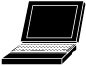
\includegraphics[width=1cm]{images/laptop.jpg}};
            \node (pc1) [anchor=north] at (10,0) {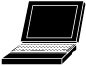
\includegraphics[width=1cm]{images/laptop.jpg}};
            \node (r0) [anchor=north] at (3,2) {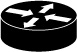
\includegraphics[width=1cm]{images/router.jpg}};
            \node (r1) [anchor=north] at (7,2) {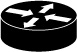
\includegraphics[width=1cm]{images/router.jpg}};

            \node [anchor=south] at (0,0) {PC0};
            \node [anchor=south] at (10,0) {PC1};
            \node [anchor=south] at (3,2) {R0};
            \node [anchor=south] at (7,2) {R1};

            \draw (pc0) -- (r0);
            \draw (r0) -- (r1);
            \draw (r1) -- (pc1);
        \end{tikzpicture}
        \begin{tabular}{ll}
            réseau & 192.168.1.0/24 \\
            PC0 & 192.168.1.10 \\
            ETH0 du routeur0 & 192.168.1.1 \\
            Réseau & 192.168.2.0/24 \\
            ETH1 de routeur0 & 192.168.2.1 \\
            ETH0 de routeur1 & 192.168.2.2 \\
            Réseau & 192.168.3.0/24 \\
            ETH1 de routeur 1 & 192.168.3.1 \\
            PC1 & 192.168.3.10
        \end{tabular}
    \end{center}
    Routes de R0:
    \begin{center}
        \begin{tabular}{|l|l|} \hline
            route 1 & \\ \hline
            route 2 & \\ \hline
            route 3 & \\ \hline
        \end{tabular}
    \end{center}
\end{itemize}









\end{document}
